\chapter{Using the HBase Java API}
%Intro\footnotemark\\
\par Lorem ipsum dolor sit amet, consectetur adipiscing elit. Aliquam facilisis massa quis orci volutpat, ut dictum tellus pulvinar. Nam vulputate diam a leo dignissim varius. Aenean nec tellus malesuada, tristique libero vitae, lacinia nibh. Donec quam libero, accumsan sollicitudin massa a, dictum gravida mauris.
\begin{spacing}{1.2}
%note en bas de page
\section{Configure the CLASSPATH in the .bashrc }
\par Lorem ipsum dolor sit amet, consectetur adipiscing elit. Aliquam facilisis massa quis orci volutpat, ut dictum tellus pulvinar. Nam vulputate diam a leo dignissim varius. Aenean nec tellus malesuada, tristique libero vitae, lacinia nibh. Donec quam libero, accumsan sollicitudin massa a, dictum gravida mauris
\\
\begin{figure}[!htb] 
\begin{center} 
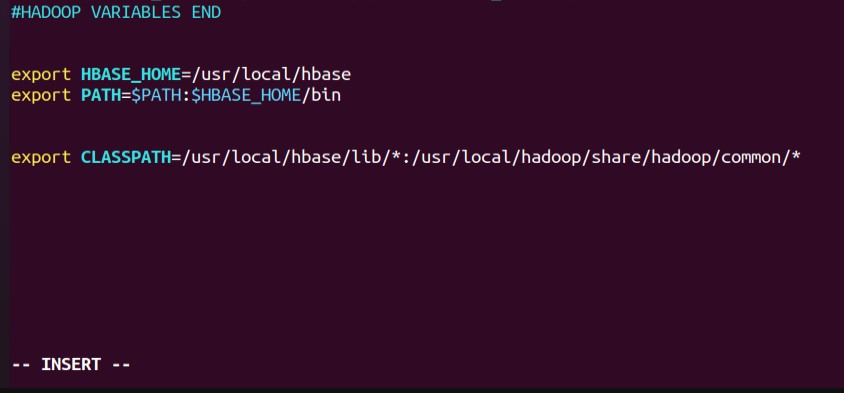
\includegraphics[width=1\linewidth]{Pictures/HBase/Using the HBase Java API/Configure the CLASSPATH in the .bashrc/Adding classpath in .bashrc} 
\end{center} 
\caption{Adding classpath in .bashrc} 
\end{figure}  \FloatBarrier
\\

\par Lorem ipsum dolor sit amet, consectetur adipiscing elit. Aliquam facilisis massa quis orci volutpat, ut dictum tellus pulvinar. Nam vulputate diam a leo dignissim varius. Aenean nec tellus malesuada, tristique libero vitae, lacinia nibh. Donec quam libero, accumsan sollicitudin massa a, dictum gravida mauris
\\
\begin{figure}[!htb] 
\begin{center} 
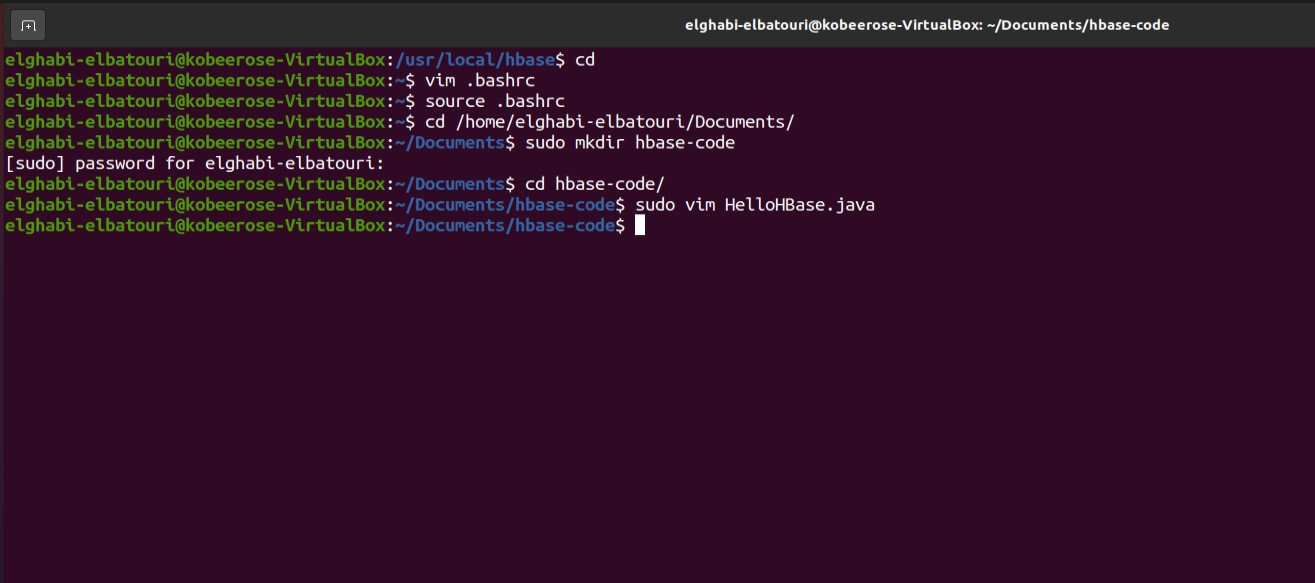
\includegraphics[width=1\linewidth]{Pictures/HBase/Using the HBase Java API/Configure the CLASSPATH in the .bashrc/Creating hbase-code repository} 
\end{center} 
\caption{Creating hbase-code repository} 
\end{figure}  \FloatBarrier
\\

\par Lorem ipsum dolor sit amet, consectetur adipiscing elit. Aliquam facilisis massa quis orci volutpat, ut dictum tellus pulvinar. Nam vulputate diam a leo dignissim varius. Aenean nec tellus malesuada, tristique libero vitae, lacinia nibh. Donec quam libero, accumsan sollicitudin massa a, dictum gravida mauris
\\
\begin{figure}[!htb] 
\begin{center} 
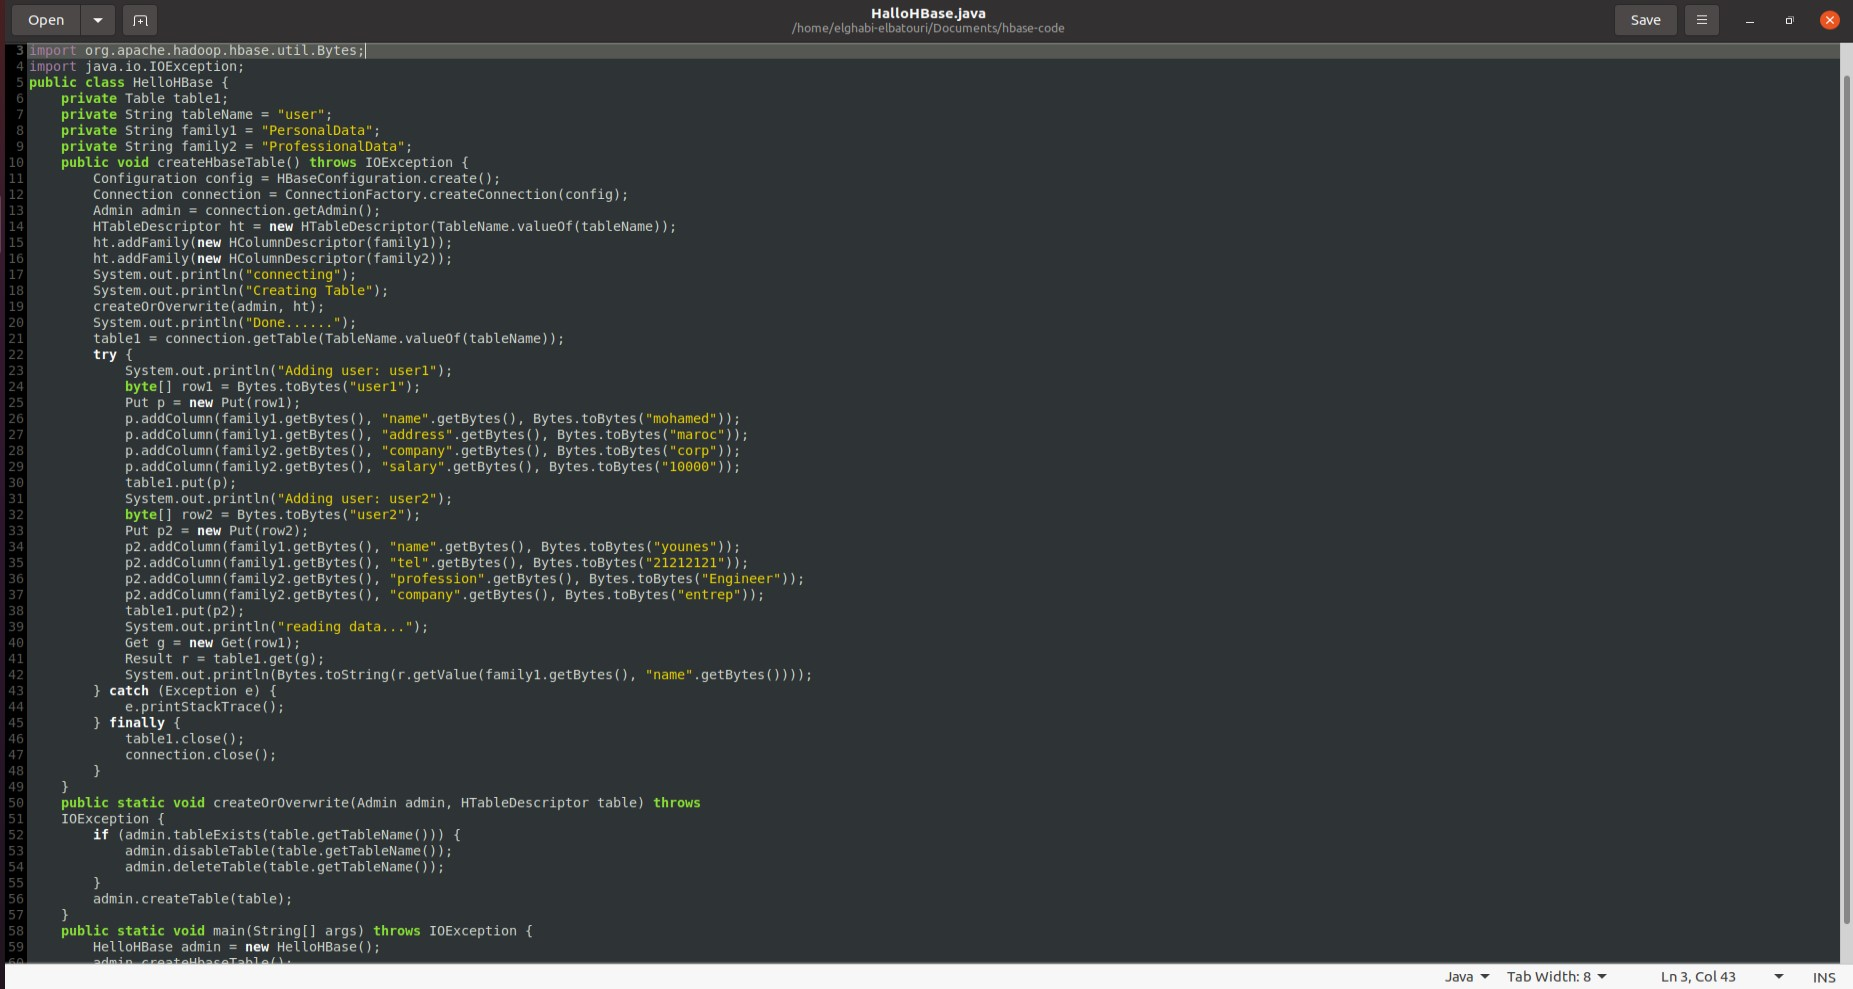
\includegraphics[width=1\linewidth]{Pictures/HBase/Using the HBase Java API/Configure the CLASSPATH in the .bashrc/HelloBase.java code} 
\end{center} 
\caption{HelloBase.java code} 
\end{figure}  \FloatBarrier
\\

\par Lorem ipsum dolor sit amet, consectetur adipiscing elit. Aliquam facilisis massa quis orci volutpat, ut dictum tellus pulvinar. Nam vulputate diam a leo dignissim varius. Aenean nec tellus malesuada, tristique libero vitae, lacinia nibh. Donec quam libero, accumsan sollicitudin massa a, dictum gravida mauris
\\
\begin{figure}[!htb] 
\begin{center} 
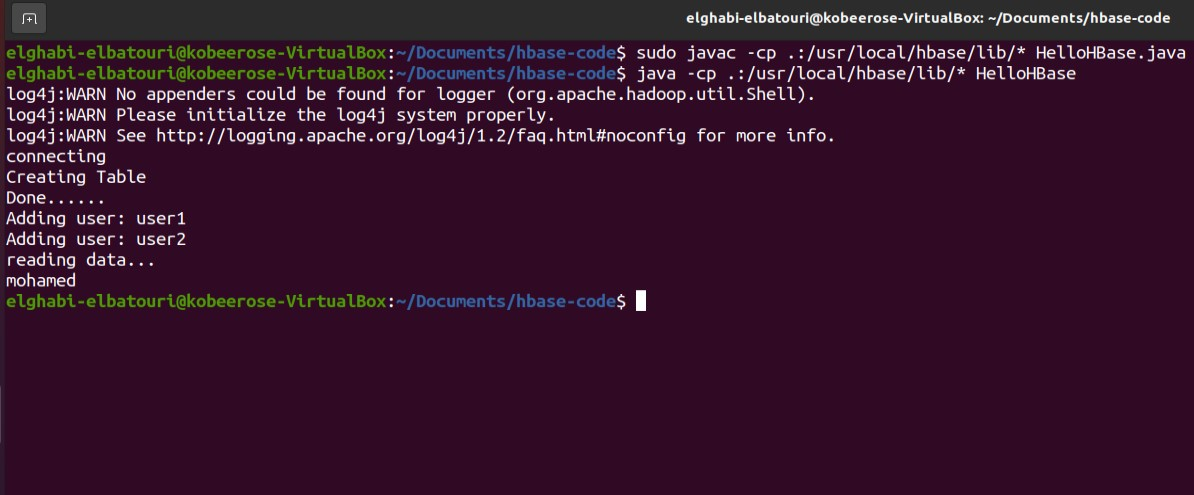
\includegraphics[width=1\linewidth]{Pictures/HBase/Using the HBase Java API/Configure the CLASSPATH in the .bashrc/Compile and run the Class} 
\end{center} 
\caption{Compile and run the Class} 
\end{figure}  \FloatBarrier
\\
\section{MapReduce on stored file }
\par Lorem ipsum dolor sit amet, consectetur adipiscing elit. Aliquam facilisis massa quis orci volutpat, ut dictum tellus pulvinar. Nam vulputate diam a leo dignissim varius. Aenean nec tellus malesuada, tristique libero vitae, lacinia nibh. Donec quam libero, accumsan sollicitudin massa a, dictum gravida mauris
\\
\begin{figure}[!htb] 
\begin{center} 
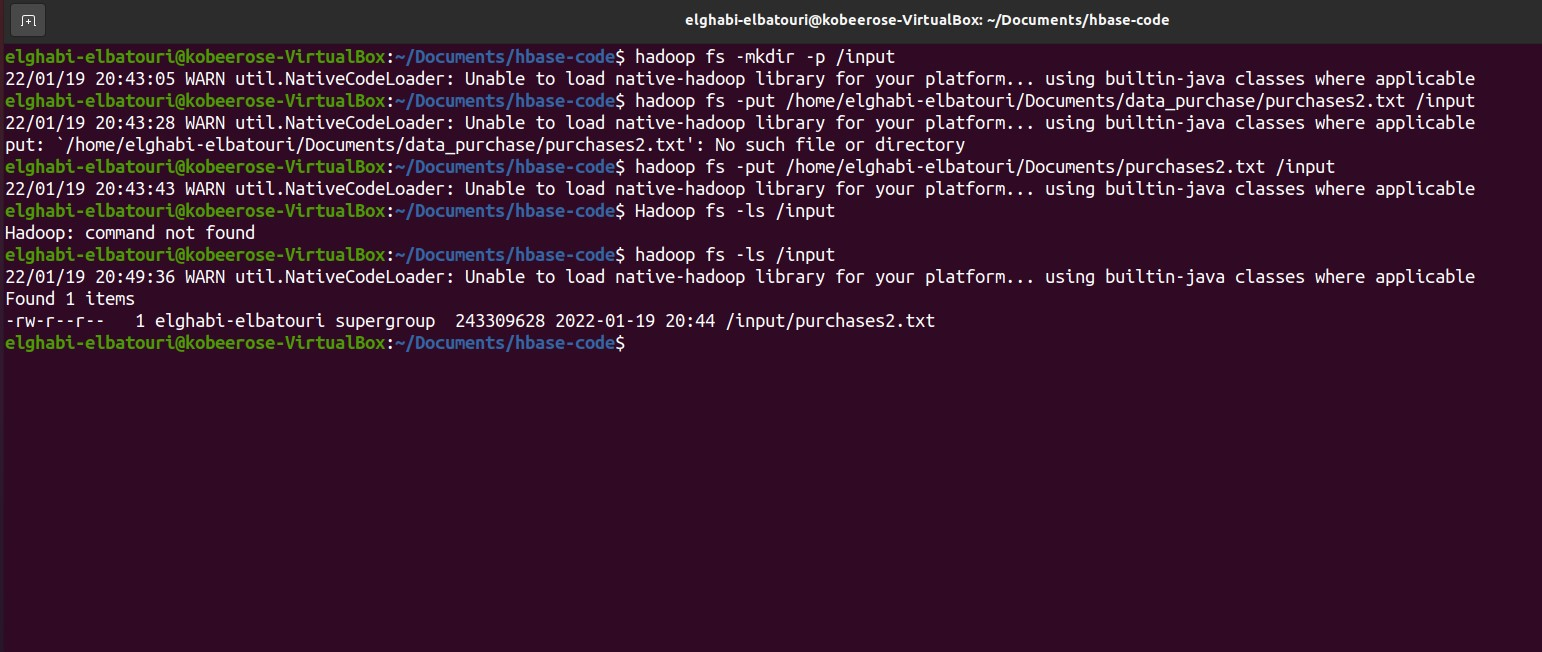
\includegraphics[width=1\linewidth]{Pictures/HBase/Using the HBase Java API/MapReduce on stored file/Putting the file into HDFS directory} 
\end{center} 
\caption{Putting the file into HDFS directory} 
\end{figure}  \FloatBarrier
\\

\par Lorem ipsum dolor sit amet, consectetur adipiscing elit. Aliquam facilisis massa quis orci volutpat, ut dictum tellus pulvinar. Nam vulputate diam a leo dignissim varius. Aenean nec tellus malesuada, tristique libero vitae, lacinia nibh. Donec quam libero, accumsan sollicitudin massa a, dictum gravida mauris
\\
\begin{figure}[!htb] 
\begin{center} 
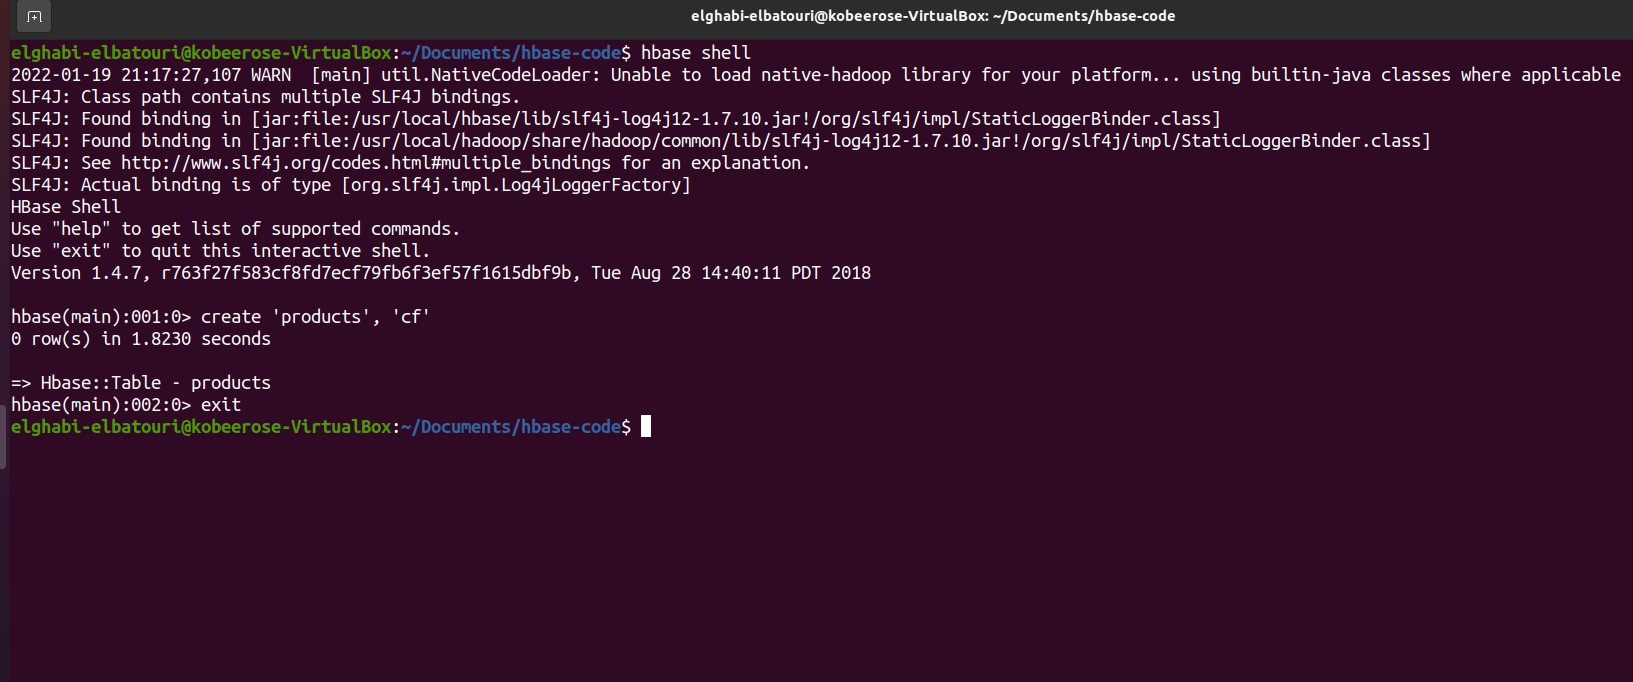
\includegraphics[width=1\linewidth]{Pictures/HBase/Using the HBase Java API/MapReduce on stored file/Create product database} 
\end{center} 
\caption{Create product database} 
\end{figure}  \FloatBarrier
\\

\par Lorem ipsum dolor sit amet, consectetur adipiscing elit. Aliquam facilisis massa quis orci volutpat, ut dictum tellus pulvinar. Nam vulputate diam a leo dignissim varius. Aenean nec tellus malesuada, tristique libero vitae, lacinia nibh. Donec quam libero, accumsan sollicitudin massa a, dictum gravida mauris
\\
\begin{figure}[!htb] 
\begin{center} 
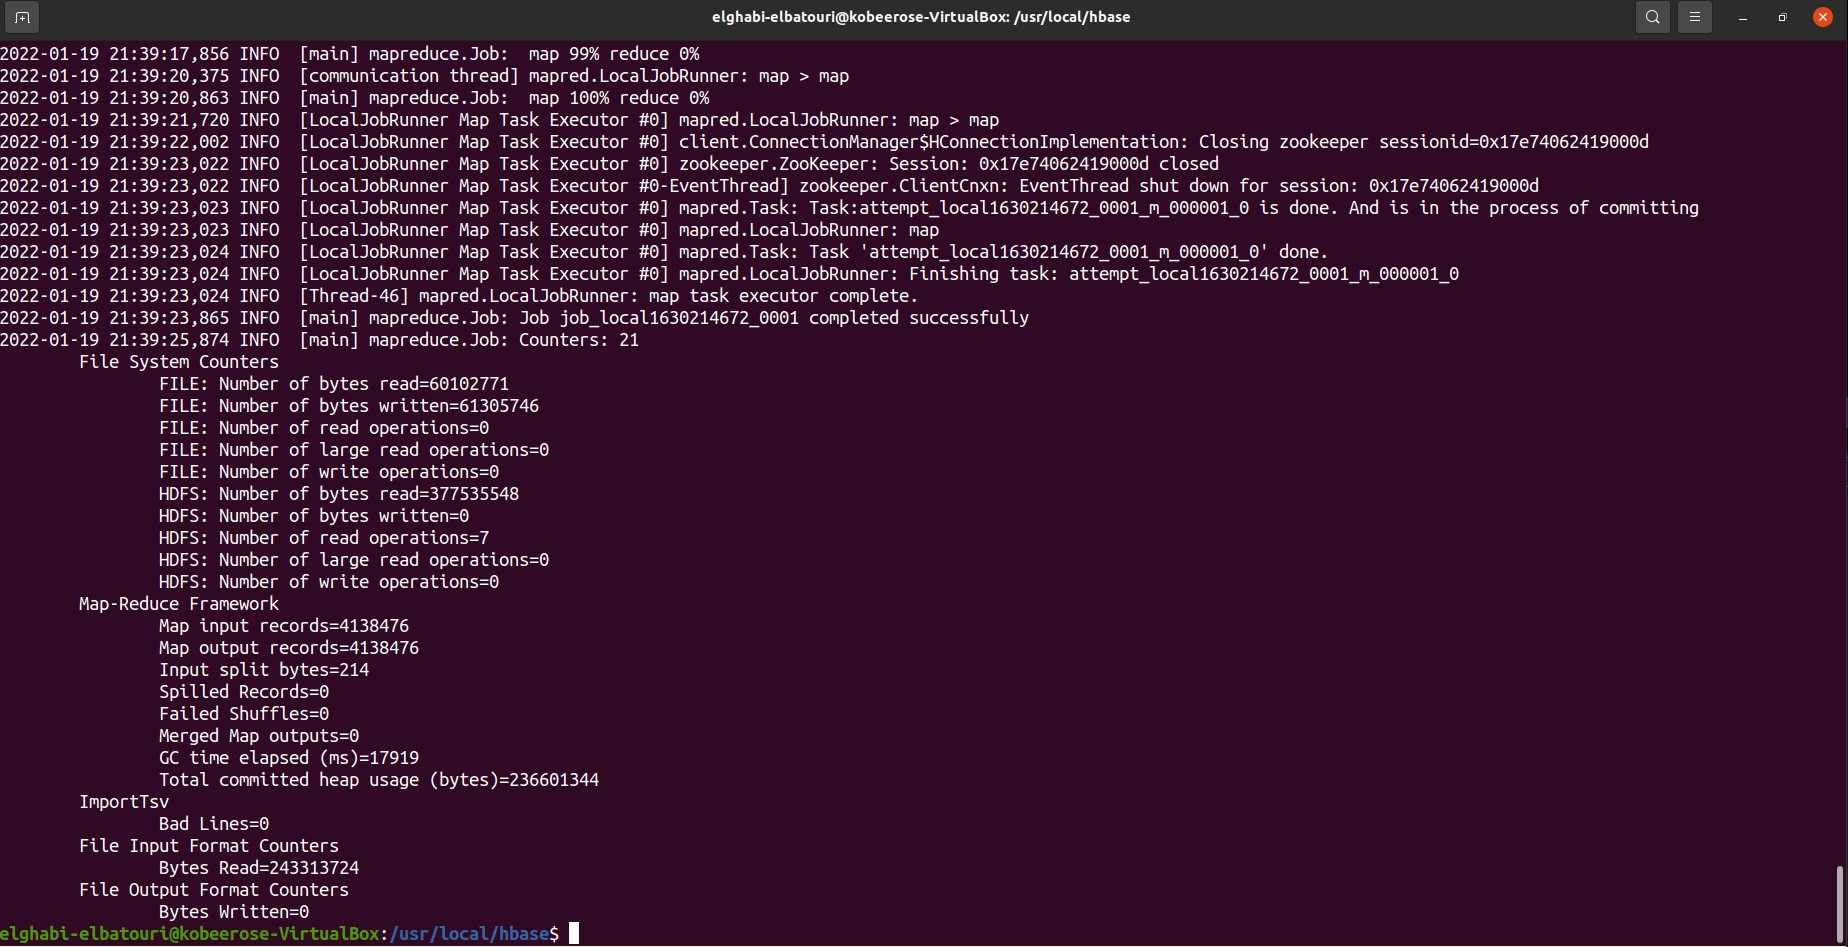
\includegraphics[width=1\linewidth]{Pictures/HBase/Using the HBase Java API/MapReduce on stored file/MapReduce on the stored file} 
\end{center} 
\caption{MapReduce on the stored file} 
\end{figure}  \FloatBarrier
\\

\par Lorem ipsum dolor sit amet, consectetur adipiscing elit. Aliquam facilisis massa quis orci volutpat, ut dictum tellus pulvinar. Nam vulputate diam a leo dignissim varius. Aenean nec tellus malesuada, tristique libero vitae, lacinia nibh. Donec quam libero, accumsan sollicitudin massa a, dictum gravida mauris
\\
\begin{figure}[!htb] 
\begin{center} 
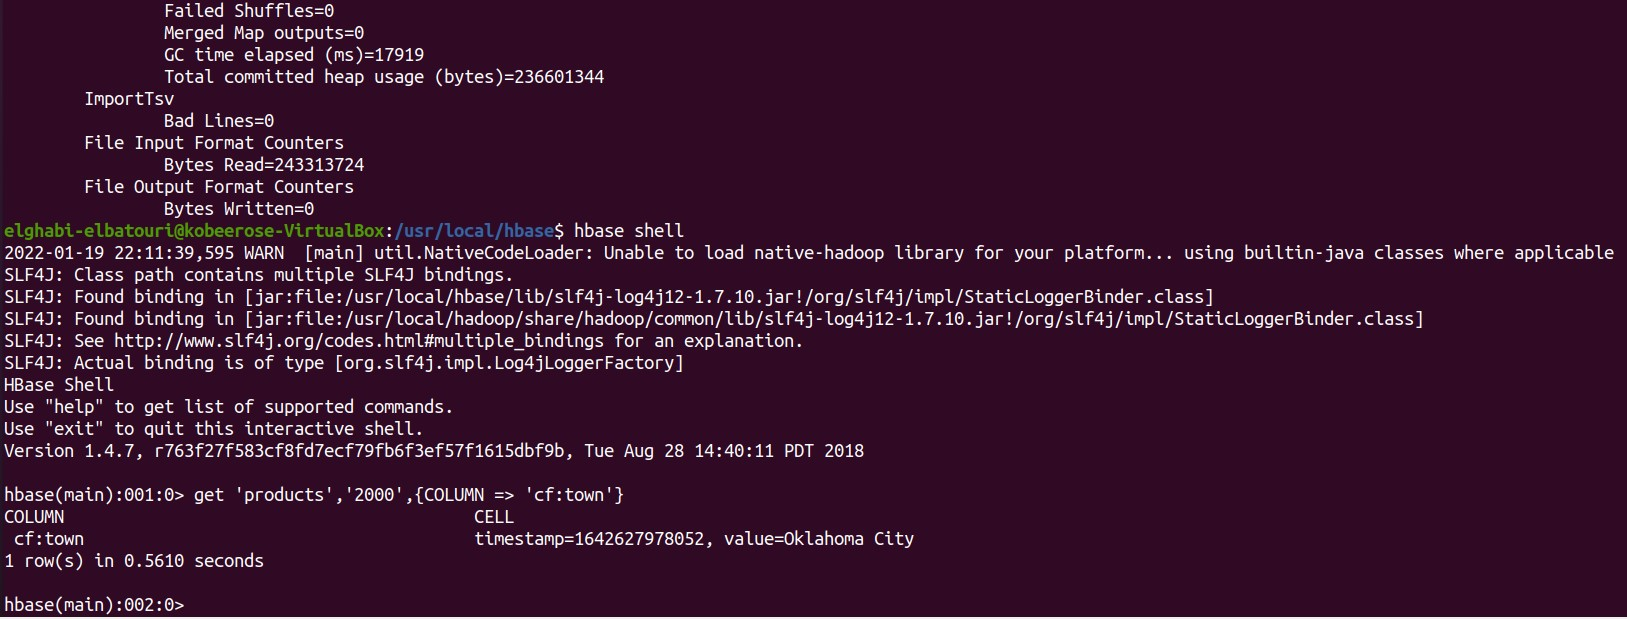
\includegraphics[width=1\linewidth]{Pictures/HBase/Using the HBase Java API/MapReduce on stored file/Verifying the Database} 
\end{center} 
\caption{Verifying the Database} 
\end{figure}  \FloatBarrier
\\

\end{spacing}